\section{Lezione 7} \hfill 10/03/2026
\subsection{Specie aliene}
Nei boschi planiziali ci sono altre specie, spesso provenienti da altre zone.\\
\textit{Specie aliena}: specie che arriva da fuori (importata, che è fuori dal suo areale) ed è pericolosa (tende a prendere il sopravvento perchè non ha limitatori naturali): può allargarsi in maniera spropositata, perchè i predatori/funghi non la conoscono.\\
\textit{Specie esotica}: specie che arriva da fuori, ma non risulta come un pericolo o problema per l'ecosistema.\\
Il termine esotico non è sinonimo di quello alieno.\\
\subsubsection{Robinia pseudoacacia - Acacia, falsa acacia, robinia}
Non è più un'aliena, perchè sono presenti i suoi nemici.\\
Si chiama Robinia dal nome del giardiniere del Re Sole (Jean Robin), che per primo l'ha portata in Europa (dal '700), da inserire nel giardino di Versailles.\\
Ha una chioma leggera verde chiara, con fiori profumatissimi che durano un mesetto (all'incirca nel mese di maggio).\\
È originaria degli Stati Uniti orientali (dei Monti Apalachi).\\
Ha diverse caratteristiche interessanti:
\begin{itemize}
    \item è una leguminosa, ovvero in grado di fissare l'azoto con i suoi tubercoli;
    \item è una tipica pioniera secondaria (cioè pioniera in suoli già esistenti, evoluti);
    \item è una miglioratrice del suolo (grazie ai suoi tubercoli radicali);
    \item cresce bene ed in fretta dove il suolo è fertile, e ha difficoltà dove il suolo non lo è;
    \item ha una capacità di moltiplicazione eccezionale;
    \item la rinnovazione da seme è molto difficoltosa, essendo un seme duro che non tende a germinare;
    \item è una pianta mellifera.   
\end{itemize}
Essendo pioniera:
\begin{multicols}{2}
\begin{itemize}
    \item ha una vita breve (meno di 100 anni);
    \item ha una forte capacità pollonifera caulinare e radicale;
    \item è eliofila.
\end{itemize}
\end{multicols}
Il suo legno:
\begin{multicols}{2}
\begin{itemize}
    \item è ottimo per la combustione;
    \item è molto duro ed elastico;
    \item ha l'alburno chiaro e durame che va dal bruno-verde-oro;
    \item è molto nervoso;
    \item ha un uso limitato come segati (se non previa vaporizzazione);
    \item viene usato per la paleria dei filari interni delle viti.
\end{itemize}
\end{multicols}
Il legname da opera viene importato dall'Ungheria, dove sono presenti specie selezionate e coltivate a fustaia.\\
Da una ventina-trentina d'anni sono presenti alcuni sui antagonisti, tipo il lepidottero Parectopa robiniella (defogliatore) o scolitidi (che attacca le robinie con almeno 15 cm DBH).\\
La gestione:
\begin{itemize}
    \item forma popolamenti puri (essendo molto aggressiva);
    \item viene gestita a ceduo semplice (avendo una capacità pollinare molto forte);
    \item non viene previsto l'uso di matricine (non serve sostituire le ceppaie che vanno a morire), anche se in alcune Regioni è comunque obbligatoria la matricinatura;
    \item i turni sono brevi (minimo 7 anni), normalmente 10-15 anni;
    \item l'incremento, in condizioni normali, è di 15-20 \unit{m^3/ha \cdot y}: È UNA MACCHINA DA LEGNO;
    \item il robinieto è una ottima serra, per la protezione di latifoglie nobili (es. ciliegio);
    \item la coltivazione ad alto fusto richiede molto spazio per le piante (almeno 10 m tra ognuna) oppure l'alternanza tra specie;
    \item dopo una nevicata intensa, la pianta si piega e non si raddrizza più (conviene tagliare e piantare nuovamente).
\end{itemize}
Essendo fortemente invasiva, la robinia è stata considerata in passato dai forestali italiani come il nemico da eliminare: per fare ciò sono stati svolti tagli (per questa specie è stato un processo favorevole, data laforte capacità pollonifera).\\
Per eliminare la robinia occorre lasciarla invecchiare (``la robinia non si sopporta''): un robinieto che può avere decine di migliaia di fusti ad ettaro si riduce in fretta autonomamente.\\
Essendo che la chioma è leggera (sotto arriva luce), la vegetazione è banale (invasive prative o le specie del bosco che c'erano prima): invecchiando, il robinieto rende favorevole la condizione delle specie sotto ad esso. Non tagliare la robinia ha un doppio effetto: favorisce l'ingresso delle specie autoctone ed impedisce la produzione di nuovi polloni.\\
In un momento di molta richiesta di energia/biomassa e la limitazione all'utilizzazione dei boschi tradizionali, il robinieto può essere una grande fonte di assortimenti legnosi di ottima qualità.\\
I robinieti sono molto frequenti perchè nel secondo dopoguerra, con l'inizio dell'industrializzazione, era una bestemmia l'abbandono della terra: per questo motivo vennero piantati polloni radicali di robinia (schemi di 4x2 o 3x2) di robinia, che dopo 7-8 anni venivano ceduati per far partire il vero robinieto.\\
In definitiva, la robinia può essere un alleato e non un problema. Se la robinia invecchia, si perde.
\begin{figure}[htbp]
     \centering
     % Prima Immagine
     \begin{subfigure}[b]{0.33\textwidth}
         \centering
         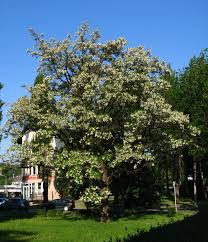
\includegraphics[width=\textwidth]{immagini/robinia_portamento.jpg}
        %\caption{}
     \end{subfigure}
     \hfill % Spazio elastico tra le immagini
     % Seconda Immagine
     \begin{subfigure}[b]{0.3\textwidth}
         \centering
         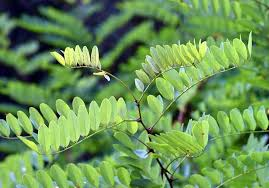
\includegraphics[width=\textwidth]{immagini/robinia_foglie.jpg}
        %\caption{}
     \end{subfigure}
     \hfill % Spazio elastico tra le immagini
     % Terza Immagine
     \begin{subfigure}[b]{0.33\textwidth}
         \centering
         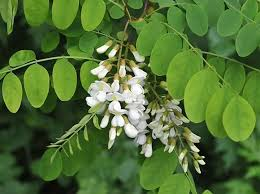
\includegraphics[width=\textwidth]{immagini/robinia_fiori.jpg}
        %\caption{}
     \end{subfigure}
     
    \caption{Robinia pseudoacacia}
     \label{fig:robinia}
\end{figure}
\subsubsection{Ailanto - Ailanthus altissima}
Anche detto ``albero del paradiso'', data la bellezza della pianta.\\
È una specie di origine cinese, è stata importata per i giardini.\\
Dato l'apparato radicale estremamente robusto e fittonante a forma di S, è stato utilizzato in passato per sistemare le massicciate ferroviarie: per questo motivo è diffuso in tutta Italia.\\
Questa specie: 
\begin{itemize}
    \item ha una capacità pollonifera radicale (molto più forte della robinia) e caulinare;
    \item è fortemente eliofila e fortemente rustica;
    \item è in gradi di colonizzare suoli estremamente primitivi;
    \item produce un'abbondatissima produzione di seme alato (samare);
    \item ha individui maschi e femmine.
\end{itemize}


le femmine si riempiono di (?)\\
si trova in tutta italia\\
È il problema , perchè non ha nemici. In passato veniva contenuto, per il gran numero di ceduazione (prop. tramite polloni radicali e non seme) -> con l ' abbandono delle campagne sono andati in seme e iniziato a propagarsi\\
sarebbe una specie da eradicare : la soluzione sarà da trovare in futuro. per contenerlo si potrebbe rendere il suolo ombreggiato, poichè molto eliofilo\\
si potrebbe utilizzarlo: legno bianco molto stabile (come il pioppo), 0,6-0,7 di densità, bianco indifferenziato, legno di media qualità per la combustione (viene piano piano accettato dal mercato). \\
le foglie sono utilizzate in farmaceutica\\
pianta mellifera (fiorisce moltissimo)\\
è una bella pianta\\
avendo il midollo vuoto, se ha delle ferite nella chioma, può entrare acqua e farlo marcire (conviene non allungare i turni, 40-50 anni max)\\
rimuoverlo sarebbe la cosa migliore\\
è stata provata la cercinatura in passato: ha avuto una percentuale comunque bassa di sopravvivenza\\
l'ailanto ha le foglie che puzzano (?)\\
maschi infiorescenza gialla e le femmina rossa\\
il futuro dei boschi planiziali e basso collinare è quello di essere invaso dall'ailanto
\subsubsection{paulonia}
la paulonia fa cagare 48\\
enormi foglie che fa, utilizzata in arboricoltura da legno (scarso successo)\\
le grandi foglie sono a rischio per defogliatori, uso di diserbante, grandinate\\
il legno è molto morbido\\
in collina cresce molto bene (problema nei colli euganei)\\
si eradica abb faciltmente, buona cap pollonifire caulinare
\subsubsection{prunus serotina, ciliegio americano}
prima della metà novecento, ci fu la ricerca della specie definitive per la produz legnosa: nel varesotto ci fu l'importazione di prunus serotina, con legno simile al nostro ciliegio\\
proveniente dagli usa orientali, forte cap poll. caulinare e radicale, serotinicità dei semi (stanno nella banca del suolo anche 20 anni, in attesa di germinare); pianta di mezza luce, tende ad essere aggressiva.\\
tutta la valle del ticino è invasa, in continua invasione\\
riconoscibile dal verde lucido, foglia simile al ciliegio, profumo simile alla mandorla\\
l'unico modo per eradicarlo naturalmente è tenere una copertura del bosco molto densa (ovvero non utilizzare il bosco)
\subsubsection{Acero negundo}
statunitense, dall'aspetto è il meno aceroso tra tutti gli aceri\\
come tutti gli aceri è pioniera di seconda tipo, molto rustica, molto resistente all'inquinamento , resiste bene alla potatura, tende a diventare invasivo\\
capacità pollonifera solo caulinare, quindi abbastanza facile da controllare
\subsubsection{albero di giuda}
scappato dai giardini, originario della palestina
\subsubsection{quercia rossa}
usata molto nel dopoguerra come alternativa alla rovere\\
quercus palustris e quercus (?)\\
quercus palustris: lobi molto più marcati della prima\\
le foglie diventano rosse in autunno\\
la ghianda è quella del film l' era ghiaciale\\
negli usa orientali, metà delle case sono costruite in legno di quercia rossa\\
fu importata data la rapida crescita\\
il legno è quasi bianco, utilizzato oggi per le bare\\
non è difficile da controllare , avendo solo la cap. pollonifera caulinare (che perde intorno ai 30 anni).\\
dove ci sono gli eucalipteti (spagna portogallo), è un problema...non è un problema nostro
\subsubsection{ligustru}
è un alberello, vicino ai giardini.\\
se non viene tagliato va  a frutto 
\\\\
tendono a costituire uno strato basso e denso, limitando la maturazione per le specie autocnote\\
\subsubsection{Amorfa frutticosa}
falsa acacia\\
quando si deve fare una utilizzazione \dots
\subsubsection{falso gelso}
in PP, vicino al Po\\
scappata dai giardiniere
\subsubsection{Spinee}
\subsubsection{pianta delle farfalle}
molto apprezzata nei giardini, molto amata dalle farfalle\\
si trovano nelle vallate alpine, lungo i corsi d'acqua
\subsubsection{piante erbacee}
possono diventare invasive, coprendo completamente e limitando la rinnovazione\\
topinambur: fusti alti più di 2 metri che tendono a coprire tutto\\
solidarum canadensis: specie montana, importata assieme ai grani/semi, \\
raoinutra iaponica: sigillo di salomone, fusto molto lungo, che si piega, foglie simili a quelle del tiglio, è stato importato dal giappone assieme ad una partita di riso, a rizomi , molto coprente, occupa qualsiasi tipo di suolo (secco, umido, pietro, corsi d'acqua)
\subsubsection{Specie medicina}
queste specie non risolvono problemi di malattie , ma risolvono specie di... , compaiono silitamente quando c'è un eccesso di azoto o condizioni di luce non consone.\\
sono rovi, sambuco, nocciolo\\
queste specie sono quasi sempre comunque presenti nel bosco, ma non in forma coprente.\\
\subsubsection{Rovi}
in collina e pianura sono per le persone comuni un problema: è disordinato e crea habitat ottimali per le specie selvatiche\\
nei boschi cedui di collina e pianura i rovi sono già presenti. nel bosco c'è poca luce, accumulo di s.o. (foglie), grossa produzione di lettiera: il taglio porta la luce da poca a tutta (la s.o. è mineralizzata in fretta, data la elevata temperatura).\\
la mineralizzazione porta un eccesso di azoto e l'elevata luce porta i rovi a diventare in eccesso. la presenza di rovi permette alle specie definitive di spuntare fuori. \\
dopo 4-5 anni dal taglio del ceduo, c'è la copertura nuovamente ed il rovo sparisce come prima\\
per combattere i rovi si potrebbe toglierlo (costoso), si potrebbe usare il glifosate (non possibile), si potrebbe tagliare il rovo una volta a fine maggio ed una volta a fine luglio (fa perdere la forza di ricaccio).
\subsubsection{nocciolo}
assolutamente coprente anche a quote più elevate (meno che del faggio)\\
\subsubsection{sambuchi}
nigra e (?)\\
se ci sono problemi, loro arrivano ed aggiustano il tutto \\